% !TeX TXS-program:compile = txs:///pdflatex/[--shell-escape]
\documentclass[conference]{IEEEtran}
%\IEEEoverridecommandlockouts
% The preceding line is only needed to identify funding in the first footnote. If that is unneeded, please comment it out.

%%%%%%%%%%%%%%%%%%%%%%%%%%%%%%%%%%%%%%%%%%%%%%%%%%%%%%%%%%%%%%%%%%%%%%%%%%%%%%%%%%
% Packages & Macros
%%%%%%%%%%%%%%%%%%%%%%%%%%%%%%%%%%%%%%%%%%%%%%%%%%%%%%%%%%%%%%%%%%%%%%%%%%%%%%%%%%
\usepackage{booktabs} % For formal tables
\graphicspath{{./graphics/}}
\DeclareGraphicsExtensions{.pdf,.jpeg,.png}


% *** GRAPHICS RELATED PACKAGES ***
%
%\usepackage[pdftex]{graphicx}

\usepackage[export]{adjustbox}
\usepackage{color}


% *** MATH PACKAGES ***
%
\usepackage{amsmath}
\usepackage{amssymb}
% A popular package from the American Mathematical Society that provides
% many useful and powerful commands for dealing with mathematics.
%
% Note that the amsmath package sets \interdisplaylinepenalty to 10000
% thus preventing page breaks from occurring within multiline equations. Use:
%\interdisplaylinepenalty=2500
% after loading amsmath to restore such page breaks as IEEEtran.cls normally
% does. amsmath.sty is already installed on most LaTeX systems. The latest
% version and documentation can be obtained at:
% http://www.ctan.org/pkg/amsmath




% *** ALIGNMENT PACKAGES ***
%
\usepackage{array}
% Frank Mittelbach's and David Carlisle's array.sty patches and improves
% the standard LaTeX2e array and tabular environments to provide better
% appearance and additional user controls. As the default LaTeX2e table
% generation code is lacking to the point of almost being broken with
% respect to the quality of the end results, all users are strongly
% advised to use an enhanced (at the very least that provided by array.sty)
% set of table tools. array.sty is already installed on most systems. The
% latest version and documentation can be obtained at:
% http://www.ctan.org/pkg/array


% *** FLOAT PACKAGES ***
%
\usepackage{fixltx2e}
% fixltx2e, the successor to the earlier fix2col.sty, was written by
% Frank Mittelbach and David Carlisle. This package corrects a few problems
% in the LaTeX2e kernel, the most notable of which is that in current
% LaTeX2e releases, the ordering of single and double column floats is not
% guaranteed to be preserved. Thus, an unpatched LaTeX2e can allow a
% single column figure to be placed prior to an earlier double column
% figure.
% Be aware that LaTeX2e kernels dated 2015 and later have fixltx2e.sty's
% corrections already built into the system in which case a warning will
% be issued if an attempt is made to load fixltx2e.sty as it is no longer
% needed.
% The latest version and documentation can be found at:
% http://www.ctan.org/pkg/fixltx2e



% *** NON FLOAT MINIPAGE ***
\makeatletter
\let\MYcaption\@makecaption
\makeatother

\usepackage{caption}
\usepackage[font=footnotesize]{subcaption}

\usepackage[inline]{enumitem}

\makeatletter
\let\@makecaption\MYcaption
\makeatother


% *** PDF, URL AND HYPERLINK PACKAGES ***
%
%\usepackage{hyperref}
\usepackage{url}
% url.sty was written by Donald Arseneau. It provides better support for
% handling and breaking URLs. url.sty is already installed on most LaTeX
% systems. The latest version and documentation can be obtained at:
% http://www.ctan.org/pkg/url
% Basically, \url{my_url_here}.


% *** MINTED COLORED CODE ***
\usepackage{minted} % Required to display colored code properly
%hack for minted to get rid of syntax error boxes
\makeatletter
\AtBeginEnvironment{minted}{\dontdofcolorbox}
\def\dontdofcolorbox{\renewcommand\fcolorbox[4][]{##4}}
\makeatother
\usepackage[utf8]{inputenc}

% *** Do not adjust lengths that control margins, column widths, etc. ***
% *** Do not use packages that alter fonts (such as pslatex).         ***
% There should be no need to do such things with IEEEtran.cls V1.6 and later.
% (Unless specifically asked to do so by the journal or conference you plan
% to submit to, of course. )

\usepackage{algorithm}
\usepackage{algorithmic}

% *** Custom Frame ***
\usepackage{mdframed}

% So footnotes for figures are properly placed
\usepackage{afterpage}

% correct bad hyphenation here
\hyphenation{op-tical net-works semi-conduc-tor}

% for left justification of text
\usepackage{ragged2e}

% for footnotes inside tables
\usepackage{threeparttable}
% helpful macros

\usepackage{xspace}

\newcommand{\hide}[1]{}
\setlength{\marginparwidth}{2cm}
%\newcommand{\comment}[1]{\marginpar{\footnotesize #1}}
%\newcommand{\comment}[1]{}
\newcommand{\comment}[1]{\textcolor{red}{[#1]}}
\renewcommand{\tilde}[0]{$\sim$}
\newcommand{\us}[0]{$\mu s$}

\newcommand{\fig}[1]{Fig.~\ref{#1}\xspace}
\newcommand{\tbl}[1]{Table~\ref{#1}\xspace}
\newcommand{\sect}[1]{Section~\ref{#1}\xspace}

% affiliation shorthand
\newcommand{\ee}[0]{$^{1}$}
\newcommand{\cs}[0]{$^{2}$}
\newcommand{\eecs}[0]{$^{1,2}$}
\definecolor{code-bgnd}{gray}{0.95}
\newcommand{\code}[1]{\colorbox{code-bgnd}{\texttt{#1}}}
%%%%%%%%%%%%%%%%%%%%%%%%%%%%%%%%%%%%%%%%%%%%%%%%%%%%%%%%%%%%%%%%%%%%%%%%%%%%%%%%%%

\begin{document}

%%%%%%%%%%%%%%%%%%%%%%%%%%%%%%%%%%%%%%%%%%%%%%%%%%%%%%%%%%%%%%%%%%%%%%%%%%%%%%%%%%
% Graphics Sources
%%%%%%%%%%%%%%%%%%%%%%%%%%%%%%%%%%%%%%%%%%%%%%%%%%%%%%%%%%%%%%%%%%%%%%%%%%%%%%%%%%
\graphicspath{{./graphics/}}
\DeclareGraphicsExtensions{.pdf,.jpeg,.png}
%%%%%%%%%%%%%%%%%%%%%%%%%%%%%%%%%%%%%%%%%%%%%%%%%%%%%%%%%%%%%%%%%%%%%%%%%%%%%%%%%%


%%%%%%%%%%%%%%%%%%%%%%%%%%%%%%%%%%%%%%%%%%%%%%%%%%%%%%%%%%%%%%%%%%%%%%%%%%%%%%%%%%
% Title & Authors
%%%%%%%%%%%%%%%%%%%%%%%%%%%%%%%%%%%%%%%%%%%%%%%%%%%%%%%%%%%%%%%%%%%%%%%%%%%%%%%%%%
\title{Hardware Description Beyond Register-Transfer-Level Languages}
%\title{Improving Hardware Programmability By\\ Exploring Beyond Register-Transfer-Level Languages}
%\title{Paper Title*\\
%{\footnotesize \textsuperscript{*}Note: Sub-titles are not captured in Xplore and
%should not be used}
%\thanks{Identify applicable funding agency here. If none, delete this.}
%}

\author{
  \IEEEauthorblockN{Oron Port}
  \IEEEauthorblockA{\textit{Electrical Engineering} \\
  \textit{Technion -- Israel Institute of Technology}\\
  Haifa, Israel \\
  soronpo@campus.technion.ac.il}
  \and
  \IEEEauthorblockN{Yoav Etsion}
  \IEEEauthorblockA{\textit{Electrical Engineering, Computer Science} \\
  \textit{Technion -- Israel Institute of Technology}\\
  Haifa, Israel \\
  yetsion@technion.ac.il}
}

\maketitle
%%%%%%%%%%%%%%%%%%%%%%%%%%%%%%%%%%%%%%%%%%%%%%%%%%%%%%%%%%%%%%%%%%%%%%%%%%%%%%%%%%


%%%%%%%%%%%%%%%%%%%%%%%%%%%%%%%%%%%%%%%%%%%%%%%%%%%%%%%%%%%%%%%%%%%%%%%%%%%%%%%%%%
% Abstract & Keywords
%%%%%%%%%%%%%%%%%%%%%%%%%%%%%%%%%%%%%%%%%%%%%%%%%%%%%%%%%%%%%%%%%%%%%%%%%%%%%%%%%%
% As a general rule, do not put math, special symbols or citations
% in the abstract
\begin{abstract}
Today's dominant hardware description languages (HDLs), namely Verilog and VHDL, rely on limited register-transfer-level (RTL) constructs. These constructs tightly couple design functionality with timing requirements and target-device constraints. As hardware designs and device architectures become increasingly more complex, these dominant HDLs yield verbose and unportable code.
To raise the level of abstraction, several high-level synthesis (HLS) tools were introduced, usually based on software languages such as C. Unfortunately, designing hardware with sequential software language semantics comes at a price; the designer loses the ability to control hardware construction and data scheduling, which is crucial in many design use-cases. 

In this paper we further extend DFiant, a Scala-based HDL that uses the dataflow model to decouple functionality from implementation constraints.
DFiant's frontend enables functional bit-accurate hardware description, while maintaining a complete timing-agnostic and device-agnostic code. DFiant bridges the gap between software programming and hardware construction, driving an intuitive functional object oriented code into a high-performance hardware implementation.

For a proof of concept, we implemented a compiler frontend for DFiant, which transforms DFiant code into a dataflow graph, and a preliminary auto-pipelining backend, which maps the graph into synthesizable Verilog code. We further implemented two test cases in DFiant: an Advanced Encryption Standard cipher block and an IEEE-754 floating point multiplier. We compared both test cases against modern design flows. Our results demonstrate that DFiant can greatly simplify hardware designs yet still maintain competitive performance.
\end{abstract}

%We defined a new language from the ground up, borrowing concepts from hardware, dataflow and software languages. The result is a strongly-typed, purely synthesizable extendable language frontend, fit for both general-purpose and high level hardware description.


\begin{IEEEkeywords}
FPGA, HDL, HLS, Dataflow
\end{IEEEkeywords}
%%%%%%%%%%%%%%%%%%%%%%%%%%%%%%%%%%%%%%%%%%%%%%%%%%%%%%%%%%%%%%%%%%%%%%%%%%%%%%%%%%


%%%%%%%%%%%%%%%%%%%%%%%%%%%%%%%%%%%%%%%%%%%%%%%%%%%%%%%%%%%%%%%%%%%%%%%%%%%%%%%%%%
% Sections
%%%%%%%%%%%%%%%%%%%%%%%%%%%%%%%%%%%%%%%%%%%%%%%%%%%%%%%%%%%%%%%%%%%%%%%%%%%%%%%%%%
\section{Introduction}
The register-transfer level (RTL) programming model paved the road for Verilog and VHDL to flourish as the leading hardware description languages (HDLs). That road, however, is steadily nearing its end as both hardware designs and devices become increasingly more complex. While the software world is striving for a "write once, run anywhere" programmability, the complexity of an RTL design implementing a given functionality may vary greatly across different FPGA and ASIC devices that incorporate various technologies and core components. Moreover, minor requirement changes may lead to significant redesigns, since RTL abstraction tightly couples functionality with timing constraints. For example, registers serve various roles such as preserving a state, pipelining and balancing a data path, deriving timed signals from an input clock, and synchronizing an input signal. This coupling between functionality, timing constraints, and device constraints leads to verbose and unportable RTL designs. 

\begin{figure}[h]
	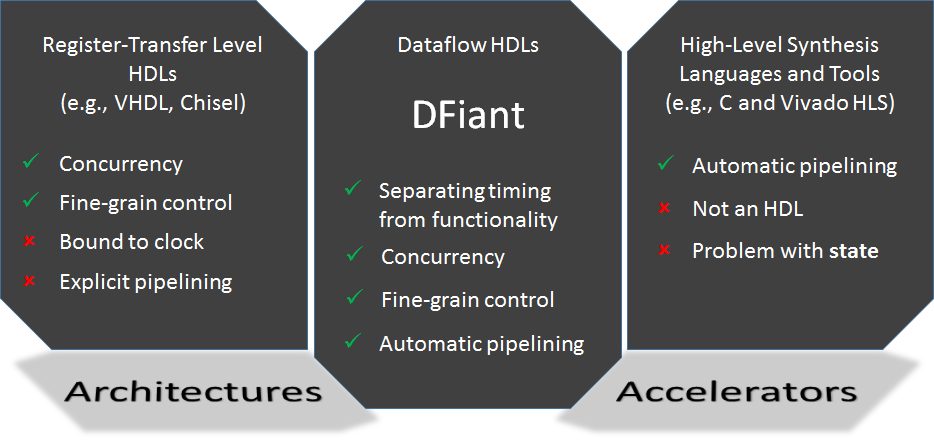
\includegraphics[width=\linewidth]{graphics/teaser}
	\caption{DFiant bridges the gap}
	\label{fig:teaser}
\end{figure}

Ongoing efforts to bridge this hardware programmability gap~\cite{Kapre2016, Nane2016, Windh2015} can be largely split into two classes: high-level synthesis (HLS) tools and high-level RTL (HL-RTL) languages.
On the one hand, HLS tools (such as Vivado~\cite{Vivado2012}, Catapult~\cite{graphics2008catapult}, and others~\cite{Kavvadias2013, synphony2015}) rely on programming languages like C and incorporate auto-pipelining and optimization mechanisms to make hardware accelerators accessible for non-hardware engineers. While this approach is successful in algorithmic acceleration domains, such languages carry von Neumann sequential semantics and thus hinder construction of parallel hardware, which is crucial for hardware design~\cite{Zhao2017}. Moreover, some trivial periodic hardware operations (like toggling a LED) are unbearably difficult to implement in HLS languages.
On the other hand, HL-RTL languages (such as Chisel~\cite{Bachrach2012}, Bluespec~\cite{nikhil2004bluespec}, PyRTL~\cite{Clow2017}, and others~\cite{Charles2016, Liu2017, jiang2018mamba, decaluwe2004myhdl, CxLang2014, Lockhart2014}) aim to enhance productivity by introducing new hardware generation constructs and semantics but do not abstract away register-level description (even Bluespec, which uses concurrent guarded atomic actions, assumes rules complete within a single clock cycle). Therefore, HL-RTL designs are still subjected to the \emph{"tyranny of the clock"}~\cite{Sutherland2012} and are bound to specific timing and target constraints.

In this paper we propose dataflow-based HDL constructs that abstract away registers and clocks. We further introduce DFiant\footnote{A preliminary version of DFiant was first introduced as a poster. The reference was removed for blind review.}, a Scala-embedded HDL that utilizes these dataflow constructs to decouple functionality from implementation constraints. DFiant brings together constructs and semantics from dataflow~\cite{le1986signal, Thuau1991, gurd1985manchester, arvind1992id}, hardware, and software programming languages to enable truly portable and composable hardware designs. The dataflow model offers implicit concurrency between independent paths while freeing the designer from explicit register placement that binds the design to fixed pipelined paths and timing constraints.

\begin{figure*}[t]
	\centering
	\captionsetup{justification=centering}
	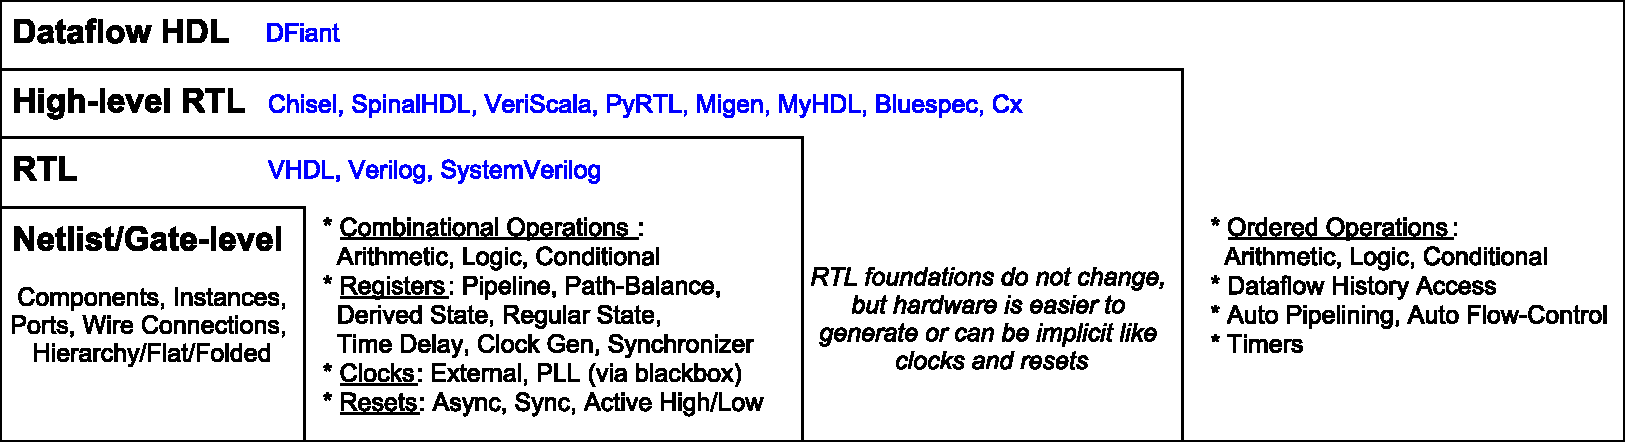
\includegraphics[width=\linewidth]{graphics/motivation.pdf} 
	\captionof{figure}{HDL abstraction layer summary (lowest=netlist, highest=dataflow)\\ Each layer subsumes the capabilities of the layer below it. Dataflow constructs replace RTL registers with their true functionality (e.g., state) or inserts them implicitly (e.g., pipelining). }
	\label{fig:motivation}
\end{figure*}

Recent related dataflow-for-hardware efforts are the Maxeler framework~\cite{Pell2011} and its MaxJ Java-based programming language, the OpenDF framework~\cite{bhattacharyya2008opendf} which is based on the CAL actor language~\cite{eker2003cal}, and CAPH~\cite{serot2011implementing}. MaxJ indeed shares common traits with DFiant, but it is tailored for its target hardware framework and is not designed to be a general purpose HDL. Both OpenDF and CAPH share similar goals with our work, but they use actors and networks to describe hardware, which is completely different than a conventional HDL composition based on component instances and port connections.

This work focuses on applying dataflow principles through the DFiant language and compiler. DFiant is \emph{not} an HLS language, nor is it an RTL language. Instead, DFiant is an HDL that provides abstractions beyond the RTL behavioral model, which reduce verbosity and maintain portable code. Since DFiant is implemented as a Scala library, it offers a rich type safe ecosystem alongside its own hardware-focused type system (e.g., bit-accurate dataflow types, input/output port types). The library performs two main tasks: first, the frontend compilation, which enforces the type-safe rule-system and constructs a dataflow dependency graph; and second, the backend compilation, which translates the graph into a pipelined RTL code and a TCL constraints file. The resulting code can be synthesized using commercial tools. 

The remainder of this paper is organized as follows. The next section details the motivation behind the dataflow HDL abstractions, and Section~\ref{sec:dfiant} which provides a general overview of the DFiant HDL language. 
Section~\ref{sec:evaluation} describes our evaluation of the DFiant language and compiler, and, finally, Section~\ref{sec:conclusion} concludes the paper.


%Interactions between DFiant types lead to hardware construction, while non-DFiant types (e.g. Integer) are considered as constants. 
 
\section{Register and State Abstraction}
\label{sec:state_abstractions}
\begin{table*}
  \begin{threeparttable}
  \captionof{table}{State Semantics Example Function, $g$: Definition and Implementations}
	\label{tbl:StateExDefImpl}
	\setlength\tabcolsep{1.5pt}
  \begin{tabular}{|c|c|c|c|c|}
  \hline 
  \textbf{Formal Definition} & \textbf{Functional Drawing} & \textbf{C++ Impl.}\tnote{†}~\tnote{‡} & \textbf{VHDL Impl.}\tnote{‡} & \textbf{DFiant Impl.} \\ 
  \hline
	\begin{minipage}[b][3.2cm][c]{0.21\linewidth}
    {\fontsize{8}{8}\selectfont
		\begin{equation}
			\nonumber
      \begin{split}
			&g:(i_{n})_{n\in \mathbb{N}}\rightarrow (a_n,b_n,c_n)_{n\in \mathbb{N}}\\  
      &\triangleq\left\{
      \begin{aligned}
      a_k &= i_k+5 & k\geq 0\\ 
      b_k &= i_k+i_{k-1} & k>0 \\   
      b_k &= i_k+0  & k=0 \\
      c_k &= i_k+c_{k-1} & k>0  \\ 
      c_k &= i_k+0 & k=0
      \end{aligned} 
      \right.
      \end{split}
		\end{equation}
    }
	\end{minipage}
  &
	\begin{minipage}[b][3.2cm][c]{0.18\linewidth}
    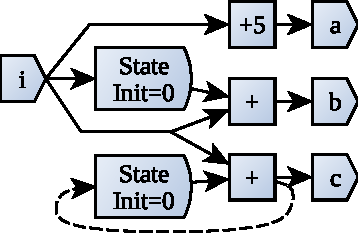
\includegraphics[width=\linewidth]{graphics/gFuncDraw.pdf}
  \end{minipage}%
  &
	\begin{minipage}[b]{0.14\linewidth}
		\begin{minted}[autogobble,tabsize=2,fontsize=\fontsize{8}{8}\selectfont]{c}
      void g(int i,
             &a,&b,&c){
        static int î=0;
        static int C=0;
        
        a = i + 5;
        b = i + î;
        î = i;
        c = i + C;
        C = c;
      }
		\end{minted}
	\end{minipage}
	&
	\begin{minipage}[b]{0.21\linewidth}
		\begin{minted}[autogobble,tabsize=2,fontsize=\fontsize{8}{8}\selectfont]{vhdl}
      g : process(clk)
        variable î : integer:=0;
      begin
        if rising_edge(clk)
        begin
          a <= i + 5;
          b <= i + î;
          î := i;
          c <= i + c;
        end; 
      end process;
			\end{minted}
	\end{minipage}
	&
	\begin{minipage}[b]{0.23\linewidth}
		\begin{minted}[autogobble,tabsize=2,fontsize=\fontsize{8}{8}\selectfont]{scala}
      def g(i : DFSInt[32]) = 
      {
        
        
        
        val a = i + 5
        val b = i + i.init(0).prev
        val c = DFSInt[32]
        c := i + c //prev optional
        (a,b,c) //tuple of three
      }
		\end{minted}
	\end{minipage}
  \\
  \hline
  \end{tabular}
  \begin{tablenotes}
    \item [†] Some type annotations were removed for brevity.
    \item [‡] \textbf{î} and \textbf{C} represent previous state values of \textbf{i} and \textbf{c}, respectively.
  \end{tablenotes}
  \end{threeparttable}
\end{table*}%

In the previous section we compared implementations of a pure (stateless) function, $f$. Typical designs, however, possess a state that is implemented via clocked registers. Registers have other functional roles, such as pipelining a data path, deriving timed signals from an input clock, and synchronizing an input signal. We believe that by avoiding explicit register use, we can design without, or very little, clock dependency. 

In this section we classify various register use-cases, and present their DFiant functional counterpart. The classifications are divided into three main categories: \textit{synchronous technology backend}, \textit{synchronous technology interface}, and \textit{state}. For the state classification, we also explore an impure function, $g$, and compare its implementation in VHDL, C++, and DFiant (see Table~\ref{tbl:StateExDefImpl}).

%Clocked registers have various functional roles, yet all appear the same in modern HDL designs. 
%The main reason is that devices have very small number of IO ports, measurable in the hundreds, while modern designs process trillions of bps. Designs are This, of course, forces existance of state, since pure functions must receive all inputs  . Therefore, it is impossible to avoid state in a full (\textit{top}) system hardware description. 
%When HLS abstract away the clock, it is left to the code analysis to classify what variable hold state.

\subsection{Synchronous Technology Backend}
Registers are often forced upon the design due to a synchronous technology choice. Since they are unrelated to the functional requirement, DFiant has no constructs to express them, and relies on its compiler to implement them properly based on the functional requirements and design constraints.
We differentiate between the following backend register uses:
\subsubsection{Pipelining}
DFiant auto-pipelines the design by inserting registers to split long combinational paths. The amount of pipelining is determined by designer-specified constraints, such as the maximum path cycle latency, or the maximum propagation delay between registers.
\subsubsection{Synchronizers}
Sampling clock domain crossing (CDC) or asynchronous signals is exposed to metastability. Synchronizers, often composed of registers, are used to mitigate its effect and bring the design to the proper reliability. Since we aspire for a clockless design frontend, we want the synchronizers to be implicit. Currently, DFiant only supports a single clock backend, and does not require synchronizers. Further research may explore other backend options.

\subsection{Synchronous Technology Interface}
Functional design requirements are often accompanied by synchronous input/output (IO) timing constraints such as clocked protocol interfaces or real-time restrictions. However, these constraints only effect the interface, and are unrelated to the design core. To maximize design portability, we apply legacy constructs solely in the periphery, while keeping the design core coded in dataflow. DFiant exposes a frontend bridge across legacy RTL constructs and its dataflow types. We differentiate between the following synchronous signaling:
\subsubsection{External IO and Blackbox Interfaces}
External IOs that are exposed to the top design hierarchy, or blackboxes that are exposed to the internal design core, may impose synchronous protocols (e.g., data is valid one clock cycle after address is set). DFiant supports legacy RTL constructs to synchronously interface external IOs and instantiate blackboxes. 
%We implemented a preliminary interface between DFiant and Chisel, allowing us to tap into Chisel's hardware generation and cycle accurate simulations.
\subsubsection{Timers}
Timers are design constructs for outputting real-time signals, or creating derivations of timed signal inputs. For example, a target device is fed by a 100MHz clock and we want to output a UART stream at 10Mbps or toggle a led at 1Hz. Instead of directly applying registers or clock generation components, we can create functional representation of their timed use-cases. Currently, DFiant supports timers with legacy RTL constructs. This work may be expanded to include functional timers.

\subsection{State}
State occurs when we require access to (previous) values which are no longer available on a function's inputs (e.g., cumulative sum or a state-machine's state). Table~\ref{tbl:StateExDefImpl} introduces a state function, $g$, and its implementation in C++, VHDL, and DFiant. The C++ implementation uses the \code{static} keyword to create variables that maintain the history of \code{i} and \code{c}. Because a static variable saves its value for every call of \code{g}, the C++ implementation cannot be used in the same design more than once. The VHDL implementation invokes registers (behaviorally) to save the state. Unfortunately, registers not only save the state, but also enforce specific cycle latencies. Furthermore, both C++ and VHDL declare additional variables and place extra assignments just to save the state. DFiant overcomes all these issues and in a less cumbersome way.

The DFiant state abstraction is achievable via the \code{.prev} construct, to summon the previous dataflow variable value, and also the construct \code{.init(value)}, to create an initialized dataflow variable. The \code{:=} assignment operation is available for a mutable dataflow variable such as \code{c} (see Section~\ref{sec:mutability}). The creation of \code{c} carries within it an implicit assignment \code{c := c.init(0).prev}, which makes the next assignment of \code{c}, \code{c := i + c}, equivalent to \code{c := i + c.init(0).prev}. This is possible due to the following semantics: \textit{previous values change at the end of the DFiant code} (similarly to signal update semantics in VHDL processes). One advantage is that the code resembles its RTL counterparts, but less verbose. Another advantage is that any type of state component, like the Muller C-element\cite{muller1957theory}, can be applied with DFiant as a frontend (note that the functional drawing in Table~\ref{tbl:StateExDefImpl} has no register drawn).

%entire design or process loop semantics. DFiant variables are implicitly static.
%Functionally a register is a memory with a single write port and unlimited

We differentiate between two kinds of state: \textit{derived state}, and \textit{regular state}. Addressable memory pools also hold state, but we currently classify them as blackboxes. %Future work may provide dedicated functional abstractions for such components as well.

\subsubsection{Derived State} 
A derived state is a state whose current output value is \textit{independent} of its previous value. For example, calculating output \code{b} of function \code{g} requires summoning previous value of \code{i}. 

\subsubsection{Regular State} 
A regular state is a state whose current output value is \textit{dependent} of its previous state value. For example, the cumulative sum output, \code{c}, of function \code{g} is dependent on the old sum value. 

The two types of state differ heavily in performance improvement when the design is pipelined. A path from \code{i} to \code{b} can produce a token for every clock tick, and if we pipeline the addition operation to increase the maximum frequency, the maximum throughput will increase as well. Contrarily, a path from \code{i} to \code{c} also depends on the previous value of \code{c}, and if we pipeline the addition operation of that path, the extra latency may even decrease the throughput. Furthermore, \code{i} is forked into several paths, and  abides by the slowest path throughput. 

Regular state causes bottlenecks in many systems. For instance, a processor's program counter (PC) register manifests as a regular state. The processor pipeline can only be improved thanks to a speculative mechanism that predicts the next PC value to prefetch instructions (e.g., PC+4 for a branch-not-taken prediction). In case of a miss-prediction, other mechanisms take place. Further research may expand DFiant's abstractions, and solve such problems functionally.

%\subsubsection{Speculated State} 
%A speculated state is a regular state that can generate a new speculative value when the actual next value is unavailable.

%In some cases a regular state limits the throughput too much. For example, a program counter (PC) register for a microprocessor pipeline. If we state dependent on the PC as a regular state, it won't be possible for the pipeline to handle more than one instruction at a time. A known solution for this is to speculate on the next value of PC (good guess is branch not taken). If we guessed wrong the pipeline should ignore the prefetched instructions and restart from where the branch occurred. This allows us to generate new speculative tokens of PC, without waiting for the pipeline to supply the vi

%There is no actual dataflow feedback. 

%\section{Related Work}
\label{sec:related_work}
%Raising hardware design abstractions has well known benefits \cite{coussy2009guest}, \cite{coussy2009introduction}. Nonetheless, HLS  still do not win vs VHDL. Martin, et al.~\cite{Cong2011} explain why past generations of HLS tools were not successful and what is required of new languages and tools. Gajski, et al. \cite{gajski2010input} and Hofstra and Matthijs \cite{hofstra2012comparing} compare HDL characteristics.

%DFiant is a direct continuation of our previous work \cite{Port2015}. 

Recent studies~\cite{Kapre2016}\cite{Nane2016}\cite{Windh2015} surveyed a variety of HDLs and HLS tools. Neither survey had explicit conclusion which tool or language should be used for hardware design. Earlier, we focused on comparing DFiant to VHDL and C++-based HLS. In this section, we further contrast DFiant to a few key hardware design languages and tools.

%Why unlike chisel. Chisel is advanced RTL. Compiled to Chisel.
%To be completed. Main focus: Recent HLS and DSL surveys, Maxeler, Chisel/SpinalHDL, Vivado HLS, Bluespec, Synflow(Cx), OpenCL, SystemVerilog SystemC. MyHDL.

%We have classified the related HDL and HSL tools into five categories, examined them against the limitations we described in \ref{chap:motivation}, and summarized the results into \ref{tbl:HDLs comparison}. The categories are: Native HDLs, Advanced HDLs, Functional HDLs, HLS Tools and Asynchronous HDLs. The following sections give more details for each category and language.



%\subsection*{System C} 
%This category of HDLs refers to modern HDLs which were not developed to provide a high level of synthesis, but to have less verbose and more easily generated RTL code, with higher level device-agnostic language constructs (FIFOs, BRAMs, etc.).
%Our work does recognize the importance of high-level functional constructs. However, we believe that burdening the designer with low level coding, such as the need to explicitly use registers to pipeline the design (which is a target specific element), is inefficient.
\paragraph*{\bf \em Chisel, SpinalHDL, and VeriScala}
Chisel~\cite{Bachrach2012}, SpinalHDL~\cite{Charles2016}, and VeriScala~\cite{Liu2017} are Scala-based libraries that provide advanced HDL constructs. When compared to DFiant, all three DSL libraries resemble RTL semantics by implicitly or explicitly acknowledging existence of clocked registers, and do not auto-pipeline designs. Moreover, DFiant is an early-adopter of new Scala features such as literal types~\cite{TypeLevelScala} and operations~\cite{singleton-ops}, which further improve type safety (e.g., a \code{DFBits[5].bits(Hi,Lo)} bit selection is compile-time-constrained within the 5-bits vector width confines).

%\paragraph*{\bf \em Chisel and SpinalHDL} 
%Both Chisel and SpinalHDL~\cite{Charles2016} are Scala-based libraries that provide advanced HDL constructs. SpinalHDL focuses on a more accurate hardware description (e.g., multiple clock domains), while Chisel focuses on providing cycle accurate simulation alongside its HDL constructs (via C++ test code generation). Both libraries resemble RTL semantics and do not auto-pipeline designs. 
%DFiant also imposes a tighter type safety, and raises most compilation errors to be asserted at the Scala compile-time.
%DFiant simulation can be executed within the Scala IDE, including breakpoints, watches, and console printouts. 

\paragraph*{\bf \em Synflow Cx} 
Synflow developed Cx~\cite{CxLang2014} as a designer-oriented HDL with new language semantics that better fit hardware design than the classic C syntax.
However, the concurrency in Cx limits dataflow description flexibility. A \code{fence} statement is required to force a new cycle. This statement affects all variables within a \code{task}. To avoid this, separate tasks are required, which limits functional clustering in a single task.
Moreover, Cx is not object-oriented and has a limited type-system.

\paragraph*{\bf \em MyHDL}
MyHDL~\cite{decaluwe2004myhdl} is a Python-based HDL. MyHDL favors verification capabilities over purely synthesizable hardware constructs, in contrary to our approach in DFiant. Since MyHDL is based on Python, it also lacks type-safety. MyHDL does not support automatic pipelining.

\paragraph*{\bf \em Bluespec} 
Bluespec uses concurrent guarded atomic actions to create rules that derive hardware construction. Bluespec's rules are atomic and execute within a single clock cycle. Consequently, the rule semantics bound the design to the clock, and if the design does not meet timing constraints, the rules system must be modified. 
%Furthermore, Bluespec's rules are not very intuitive to hardware designers, who are usually dataflow oriented. Making a mistake in the rules system may lead to guess work locating the missing or interrupting rule.
%While it may give a high productivity in some domains, it is not as easy for all general purpose hardware designs.
%In fact, Bluespec was the first source of inspiration for this work.

\paragraph*{\bf \em Vivado HLS} 
Vivado HLS~\cite{Vivado2012} is a mature tool that helps achieve high productivity in some domains. Nevertheless, it is not accepted as a general purpose HDL, since its C/C++ semantics are unfitting~\cite{Zhao2017} and its SystemC synthesizable constructs provide roughly identical capabilities of traditional HDLs~\cite{gajski2010input}.

\paragraph*{\bf \em Maxeler} 
The Maxeler framework~\cite{Pell2011} and its MaxJ Java-based programming language take part in acceleration systems. MaxJ is dataflow-centric, same as DFiant, but is tailored for its target use-case and does not fit as a general purpose HDL.

\begin{figure}[h]
	\vspace*{-3ex}
	\centering
	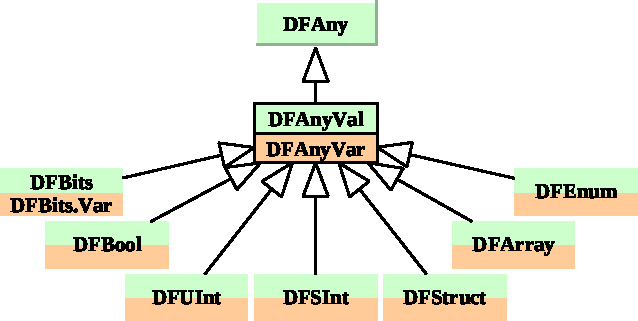
\includegraphics[scale=0.7]{graphics/Inherit.pdf} 
	\captionof{figure}{DFiant dataflow types: simplified inheritance diagram}
	\label{fig:Inherit}
\end{figure}

%\setalgorithmicfont{\small}
\begin{figure*}[h]
  \centering
  \begin{subfigure}[b]{0.5\textwidth}
    \begin{minted}[tabsize=2,gobble=3,frame=single,framesep=2pt, fontsize=\fontsize{7}{8}\selectfont]{Scala}
    class AES_DFKeySchedule(Nk: Int, Nb: Int, Nr : Int) 
      extends AES_DFWords(Nb*(Nr+1)){
      val Rcon = Array[Int](0x00000000, ...)
      def KeyExpansion(key : AES_DFKey): Unit = {
        val temp = AES_DFWord()
      
        for (i <- 0 until Nk)
          this(i) := key(i)
      
      
      
        for (i <- Nk until Nb*(Nr+1)) {
          temp := this(i-1)
          if (i % Nk == 0)
            temp := temp.RotWord().SubWord() ^ Rcon(i / Nk)
          else if ((Nk > 6) && (i % Nk == 4))
            temp := temp.SubWord()
          
          this(i) := this(i-Nk) ^ temp
        
        }
    } }
    \end{minted}
    \caption{DFiant code}
  \end{subfigure}%
%  \hfill
  \begin{subfigure}[b]{0.5\textwidth}
    \begin{minted}[tabsize=2,gobble=3,frame=single,framesep=2pt, fontsize=\fontsize{7}{8}\selectfont]{text}
    //comment line for alignment
    //comment line for alignment
    Rcon = [00000000, ...] 
    KeyExpansion(byte key[4*Nk], word w[Nb*(Nr+1)], Nk) begin
      word temp
      i = 0
      while (i < Nk)
        w[i] = word(key[4*i],key[4*i+1],key[4*i+2],key[4*i+3])
        i = i+1
      end while
      i = Nk
      while (i < Nb * (Nr+1)]
        temp = w[i-1]
        if (i mod Nk = 0)
          temp = SubWord(RotWord(temp)) xor Rcon[i/Nk]
        else if (Nk > 6 and i mod Nk = 4)
          temp = SubWord(temp)
        end if
        w[i] = w[i-Nk] xor temp
        i = i + 1
      end while
    end
    \end{minted}
    \caption{AES spec. pseudo code reference}
  \end{subfigure}
	\vspace*{-4ex}
  \caption{AES KeyExpansion code example}\label{fig:AES}
\end{figure*}

\section{The DFiant Type System}
\label{sec:type_system}
DFiant is a Scala library, hence it inherently supports type safe and rich language constructs. DFiant brings type driven development concepts to hardware design, by creating an extensible dataflow class hierarchy, with the trait \code{DFAny} at its head. 
%(similar concept to Scala's Unified Types hierarchy)
\code{DFAny} contains all properties that are common to every dataflow variable. 
%(e.g., \code{.width} represents the number of bits contained by the variable)
Fig.~\ref{fig:Inherit} illustrates a simplified inheritance diagram of DFiant's dataflow types. 

Fig.~\ref{fig:AES} depicts part of our DFiant Advanced Encryption Standard~\cite{pub2001197} (AES) cipher implementation alongside its specification pseudo code reference. The DFiant code is similar or even simpler in comparison and does not employ global functions. We compared the complete DFiant AES code to three RTL designs~\cite{das2010fully}\cite{hsing2013aes}\cite{salah2013aespipe}. DFiant provides the same functionality with 33-50\% lines of code.
Furthermore, the DFiant code is timing-agnostic and device-agnostic, thus tasking the compiler to construct the hardware fitting the target device and non-functional requirements (e.g., throughput, latency). When constrained by the appropriate target throughput, the DFiant compiler generated an RTL design that acheived better performance than the cited RTL designs.

%Since DFiant is Scala-based, the Scala IDE was utlized for debugging. It was also extremely easy to debug the code step-by-step using
%watches and console printouts. This would have been impossible to do in native HDL
%languages like VHDL and Verilog. After we fixed everything to work in software debugging backend, we have compiled the design to verilog using the hardware construction
%backend, and everything worked in RTL simulation as well.


%The DFiant type system provides the following features:
%\paragraph*{\bf \em Bit-Accurate Operations and Data Structures} 
%All DFiant's dataflow types are bit-accurate and structurally static, with their bit-width set upon construction (e.g., \code{DFBits[5]} is a 5-bit vector). Operations between dataflow variables produce a bit-accurate result with the proper type inference. For example, an addition between an unsigned 5-bit variable (\code{DFUInt[5]}) and a signed 10-bit variable (\code{DFSInt[10]}) produces an adder that can be implicitly converted to a 10-bit signed variable, if carry is not required, or an 11-bit signed variable by explicitly invoking \code{.wc} from the addition.
%
%DFiant also allows operations between dataflow types and their corresponding Scala numeric types, by treating the Scala numeric types as constants (e.g., addition between \code{DFSInt} and \code{Integer} variables). A constant in the dataflow graph is a node that can produce infinite tokens of the same value.   
%
%\paragraph*{\bf \em Mutability} 
%\label{sec:mutability}
%DFiant supports dataflow variables mutability via the \code{:=} operator. Do not confuse with Scala-level mutability which is enabled by using \code{var} instead of \code{val}. Each dataflow class has two variations: an immutable class, which inherits from \code{DFAny\textbf{Val}} and a mutable class, which inherits from \code{DFAny\textbf{Var}} and accepts \code{:=}. The difference between the types enforces an immutable right-hand-side (RHS), where required, and a mutable variable creation. Consider, for instance, the DFiant implementation of \code{g} in Table \ref{tbl:StateExDefImpl}: \code{a} is immutable because it is a RHS addition between the dataflow variable \code{i} and a literal value \code{5}. Contrarily, \code{c} is mutable, since it is a dataflow variable constructor (\code{.init} constructs a new initialized variable, while preserving the mutability trait). 
%
%Fig.~\ref{fig:Inherit} demonstrates a dual class definition for every type  (immutable and mutable). The naming convention helps to reason about the mutability. For example, \code{DFBits} and \code{DFBits.Var} are immutable and mutable classes, respectively. Constructing a new variable via \code{DFBits} (e.g, \code{val a = DFBits[5]}) returns the mutable \code{DFBits.Var[5]}. Usually, we either receive or return an immutable type, hence we do not require annotating a type with its mutable variation. In cases where we want to return a mutable type, we annotate it as an output port (see Section~\ref{sec:io_ports}).
%
%\paragraph*{\bf \em Bit Aliasing and Casting} 
%Aliasing in DFiant enables referencing a part of a dataflow variable, by invoking \code{.bits(hiIdx, loIdx)}, which creates a bits vector alias that references the original variable at the given index parameters. Every change of a dataflow variable affects its alias and vice versa (similar to VHDL's signal aliasing). Since this function also casts the variable as \code{DFBits}, this feature is used as a raw-data cast between different dataflow types. Aliasing of an alias is also possible, while maintaining relative bits indexing. Aliasing preserves the mutability trait: an alias of an immutable variable is immutable, while an alias of a mutable variable is mutable. 
%
%\paragraph*{\bf \em Structural Composition and Generation} 
%
%\begin{figure}[h]
%  \centering
%  \begin{minipage}[b][3cm][b]{0.57\linewidth}
%    \vfill
%    \begin{minted}[xleftmargin=1.5em,linenos,autogobble,tabsize=2,framesep=1pt, frame=single,fontsize=\fontsize{7}{8}\selectfont]{scala}
%      val bits128 = DFBits[128] := 0
%      val alias64 = bits128(127, 64)
%      val alias32 = alias64(31, 0)
%      val dbl = DFDouble := 1.0
%      dbl.bits(7,0) := 0x28
%      bits128(127) := 1
%      bits128(63, 0) := dbl.bits()
%      alias32(16, 8) := 0x57		    
%    \end{minted}
%    \vfill
%    \subcaption{DFiant code}
%  \end{minipage}%
%  \hfill
%  \begin{minipage}[b][3cm][b]{0.40\linewidth}
%    \centering
%    \vfill
%		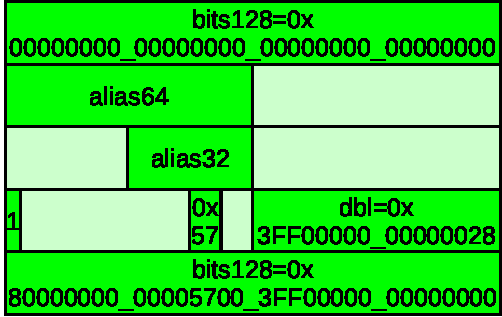
\includegraphics[width=\linewidth]{graphics/Aliasing.pdf} 
%    \vfill
%    \subcaption{Contents of \code{bits128}}
%  \end{minipage}
%  \captionof{figure}{Bit aliasing and casting example}
%  \label{fig:Aliasing}
%\end{figure}
%
%Fig.~\ref{fig:Aliasing} demonstrates aliasing code and its effect on the contents of a dataflow variable (\code{bits128}). Each line code does as follows:
%\begin{enumerate}
%  \item Constructs a new 128-bit vector, \code{bits128}, and clears all its bits.
%  \item Creates a new alias, \code{alias64}, which references the most significant 64 bits of \code{bits128}. Since \code{bits128} is a \code{DFBits} variable, there is no need to invoke \code{.bits()}, and we can apply the required indexes directly.
%  \item Creates a new alias, \code{alias32}, which references the least significant 32 bits of \code{alias64}, which reference bits 64 to 95 of \code{bits128}.
%  \item Constructs a new double precision floating point dataflow variable, \code{dbl}, and initialize its value as \code{1.0} (hexadecimal value of \code{0x3FF00...0}).
%  \item Modifies the least significant byte of \code{dbl}.
%  \item Sets the most significant bit of \code{bits128}.
%  \item Assigns \code{dbl} to the least significant 64 bits of \code{bits128} through casting. All the bits of \code{dbl} are selected because \code{.bits()} is invoked without index parameters.
%  \item Modifies a byte of \code{bits128}.
%  
%\end{enumerate}
%
%
%DFiant expands traditional structural composition capabilities by utilizing Scala's object oriented features such as inheritance and polymorphism, as well as finite loops and recursive composition. The hierarchical compositions provide the scope and dependencies for the dataflow variables. The hierarchy itself is transparent to the dataflow graph, as if the entire design is flattened, inlined, and unrolled. Therefore, hierarchies in DFiant are synthesizable, highly reusable, and do not affect the design performance (may affect compilation time). Different composition examples are available in Table~\ref{tbl:Box}.
%
%\paragraph*{\bf \em IO Ports} 
%\label{sec:io_ports}
%The class \textit{Box} from Table~\ref{tbl:Box} can also be coded as demonstrated in Fig.~\ref{fig:IOBox}. The annotation \code{DFVar $<>$ Dir} controls \textit{DFVar}'s access by encapsulating the variable with the dataflow port class, \code{DFPort}: an \code{IN} port can only be read (immutable), while an \code{OUT} port can only be modified (unreadable). DFiant has implicit conversions in place that selectively converts between \code{DFPort} and \code{DFAny} instances, without breaking mutability rules and type safety. The port annotations match the capabilities of traditional HDLs, and are noticeably absent from HLS languages such as C++. 



\section{Leading-Zero-Counter and Shifter (LZCS) Compilation Example}
\label{sec:lzc}
In this section we provide an LZCS DFiant implementation and describe its compilation process. We begin with a pseudo code reference implementation\cite{muller2009handbook} as depicted in \fig{fig:LZC_pseudo_code}. The DFiant LZCS implementation\footnote{This code was also utilized to implement FPMul in DFiant} is very similar to the pseudo code reference, as can be seen in \fig{fig:LZC_DFiant_code}.
\begin{figure}[h]
\begin{algorithm}[H]
  \caption*{Combined leading-zero counting and shifting}
  \begin{algorithmic}
    \small
    \STATE{$k \leftarrow \left\lceil \log_2{n} \right\rceil$}
    \STATE{$x_k \leftarrow x$}
    
    \FOR{$i = k-1$ downto $0$}
    \IF{there are $2^i$ leading zeros in $x_{i+1}$} 
    \STATE{$d_i \leftarrow 1$}
    \STATE{$x_i \leftarrow x_{i+1}$, shifted left by $2^i$}
    \ELSE 
    \STATE{$d_i \leftarrow 0$}
    \STATE{$x_i \leftarrow x_{i+1}$}
    \ENDIF
    \ENDFOR
    \STATE{return $(d, x0)$}
  \end{algorithmic}
\end{algorithm}
\captionof{figure}{LZCS pseudo code reference}
\label{fig:LZC_pseudo_code}
\end{figure}

\begin{figure}[h]
  \begin{minted}[autogobble,tabsize=2,frame=single,fontsize=\small]{Scala}
    def lzcs[N](num : DFBits[N]) = {
      val k = log2Up(num.width)
      val x = DFBits(num.width) := num
      val d = DFBits(k) := 0
      
      for (i <- k-1 downto 0) {
        ifdf (x.msbits(2~^i) == 0) {
          d(i) := 1
          x := x << 2~^i
        }
      }
      (d, x)
    }
  \end{minted}
  \captionof{figure}{LZCS DFiant code}
  \label{fig:LZC_DFiant_code}
\end{figure}

When we apply \code{lzcs} on an 8-bit vector \code{num}, the DFiant frontend compiler unrolls the \code{for} loop and converts the \code{ifdf} control statements into multiplexer nodes. An equivalent unrolled code is given in \fig{fig:LZC_unrolled_code}. This code is similar to the frontend compiler's static single assignment (SSA) intermediate representation (IR) form. The DFiant frontend IR is a dataflow dependency graph as illustrated in \fig{fig:LZC_Dataflow}. We can optimize the IR design independently of the target device. For example, we can derive \code{d\_i} directly from \code{c\_i} and remove unnecessary multiplexer nodes.

\begin{figure}[h]
  \begin{minted}[autogobble,tabsize=2,frame=single,fontsize=\small]{Scala}
	val x_3 = DFBits[8] := num;	 val d_3 = DFBits[3] := 0
	val c_2 = x_3(7,4)==0;        val X_3 = x_3 << 4
	val x_2 = mux(c_2, X_3, x_3); val D_3 = d_3(2):=1
	val d_2 = mux(c_2, D_3, d_3)
	val c_1 = x_2(7,6)==0;        val X_2 = x_2 << 2
	val x_1 = mux(c_1, X_2, x_2); val D_2 = d_2(1):=1
	val d_1 = mux(c_1, D_2, d_2)
	val c_0 = x_1(7,7)==0;        val X_1 = x_1 << 1
	val x_0 = mux(c_0, X_1, x_1); val D_1 = d_1(0):=1
	val d_0 = mux(c_0, D_1, d_1)
	return (d_0, x_0)
  \end{minted}
  \captionof{figure}{LZCS unrolled code for an 8-bit input}
  \label{fig:LZC_unrolled_code}
\end{figure}

The backend compiler converts the dataflow graph to Verilog and adds pipeline registers as required to achieve the target performance.
Not all dataflow nodes cost logic and therefore do not affect performance. Bit referencing, concatenation, shifting, and assignment do not cost any hardware resources (software backend compilation can incur performance  penalty). 

The preliminary auto-pipelining backend compiler we implemented relies on an estimation database that is used to calculate each node's potential propagation delay cost. The compiler makes sure no path propagation delay surpasses the target clock period, including a fixed safe margin for additional wiring delay that may occur during placement and routing. Strategic register placement brakes down long paths but increases the path clock cycle latency. All converging paths must possess the same latency to maintain correctness (we can rely on token exchange signals to provide dependency correctness, but to achieve optimal performance we need to balance the paths' latency nonetheless).

\begin{figure}[h]
  \centering
  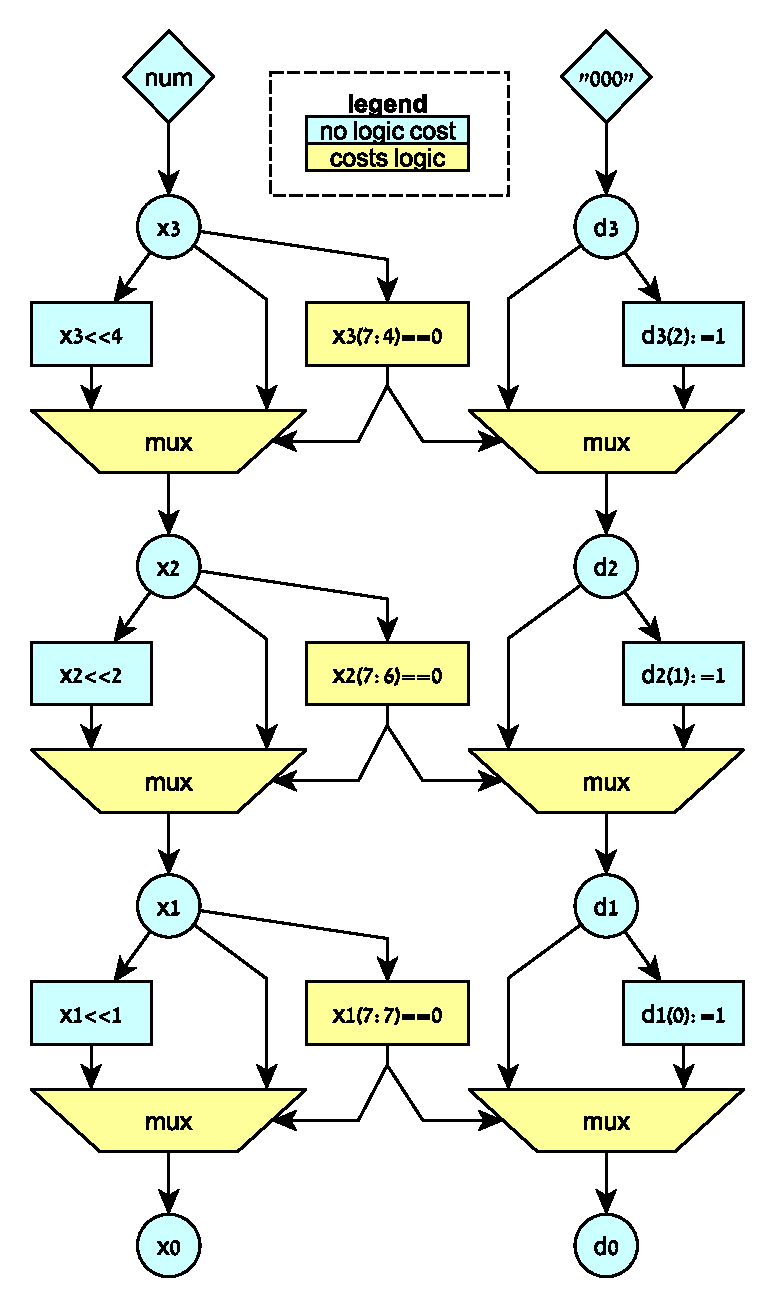
\includegraphics[width=0.8\linewidth]{graphics/lzc_dataflow.pdf}
  \captionof{figure}{LZCS IR graph for an 8-bit input}
  \label{fig:LZC_Dataflow}
\end{figure}

\section{Proof of Concept}
\label{sec:evaluation}
In this section we demonstrate DFiant frontend and backend compilers as a proof of concept the preliminary semantics of DFiant by implementing two case studies: an AES cypher, and a double precision FPMul. We compare both test cases against traditional designs, and demonstrate competing performance while simplifying code verbosity significantly. 

\subsection{Methodology}
We implemented both test cases in DFiant, constrained them by a variance of minimum frequency requirements, and compiled them to RTL. The DFiant compiler automatically pipelined the design to achieve the required minimum frequency, and generated an RTL verilog file and a TCL constraints file. For a baseline we obtained equivalent open-source RTL cores and Vivado HLS implementations, where possible. We disabled the DFiant backend support for pipelined valid/ready signaling and a blocking back-pressure, since the RTL cores did not support this capability.

We chose the following comparison metrics: the maximum clock frequency, clock cycle latency, utilizations of both look-up tables (LUTs) and flip-flop registers (FFs), and lines of code (LoC). Digital signal processing (DSP) block utilization was zero for AES and equivalent for FPMul across all designs, thus neglected from the table. a We used Xilinx Vivado to synthesize and implement the RTL design for a Virtex-7 FPGA, part number: xc7vx485tffg1761-2. The tool was configured to use default strategy for both synthesis and implementation processes. For each design, we recorded the maximum clock frequency, LUTs, and FFs. We recorded the design latency as reported by the DFiant and Vivado HLS compilers, and the RTL cores documentation. Finally, we automatically counted the LoC \cite{danial2009cloc}, applied standard score normalization (0-100) to all metrics, and assured higher values indicate better score for all metrics. Mean score of all metrics is presented as well.

\subsection{Case Study: AES Cypher}
For baseline comparison we used three AES cypher RTL designs from opencores.org: Das core \cite{das2010fully}, Hsing core \cite{hsing2013aes} and Salah core \cite{salah2013aespipe}. Additionally, we obtained a Vivado C++ HLS design~\cite{oflynn2014rapid}. All these designs are fully pipelined, meaning that in every cycle the design accepts new key and data inputs, and emits an encrypted data output, delayed by a fixed design latency.

We compiled the DFiant and Vivado HLS designs with three target clock frequencies: 200 MHz, 300 MHz, and 450 MHz. We named the designs accordingly (e.g., DFiant\_200 is the 200MHz target design). We collected the results in Table~\ref{tbl:AES_Compare_Table}, and displayed their normalized standard score in Fig.~\ref{fig:AES_Compare_Graph}. We added the supported key types quantity as a metric, since some designs support 128bit keys and do not include 192bit and 256bit keys as well. The table also includes an 'SBox BRAM Use' column, since some designs do not use memory to implement the AES SBox function.

\begin{table*}[t!]
  \centering
  \begin{minipage}[t][5cm][t]{0.62\linewidth}
    \centering
    \captionof{table}{AES Cypher RTL Designs Comparison\\(the numbering on the left associates configurations with \fig{fig:AES_Compare_Graph})}
    \label{tbl:AES_Compare_Table}
    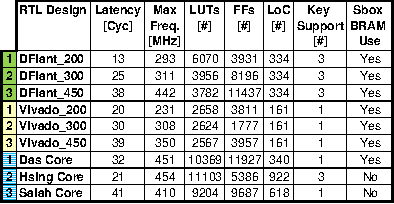
\includegraphics[scale=1]{graphics/AES_Compare_Table.pdf} 
  \end{minipage}
  \hfill
  \begin{minipage}[t][5cm][t]{0.37\linewidth}
    \centering
    \captionof{table}{FP Mult. RTL Designs Comparison\\(the numbering on the left associates configurations with \fig{fig:FP_Compare_Graph})}
    \label{tbl:FP_Compare_Table}
    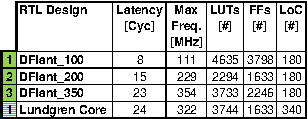
\includegraphics[scale=1]{graphics/FP_Compare_Table.pdf} 
  \end{minipage}
  \begin{minipage}[b][3.8cm][b]{0.62\linewidth}
  	\centering
    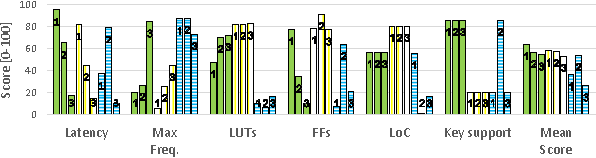
\includegraphics[height=3cm]{graphics/AES_Compare.pdf} 
    \captionof{figure}{AES cypher RTL designs score comparison (higher = better)\\ \quad}
    \label{fig:AES_Compare_Graph}
  \end{minipage}
  \hfill
  \begin{minipage}[b][3.8cm][b]{0.37\linewidth}
    \centering
    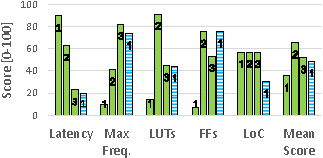
\includegraphics[height=3cm]{graphics/FP_Compare.pdf} 
    \captionof{figure}{FP multiplication RTL designs score comparison (higher = better)}
    \label{fig:FP_Compare_Graph}
  \end{minipage}
\end{table*}

The Hsing core clearly has the best performance among the different designs (but the lowest score on LUTs utilization). The primary reason it achieved this is because it uses LUTs instead of BRAMs. This enables the synthesizer to optimize the AES SBox function, and even pipeline it. DFiant uses its \code{lookupTable} library function to implement SBox, and we have yet to enable such an option for DFiant. 

Although the DFiant-generated RTL performance is not optimal, it can still  be improved without modifying the DFiant AES code, if the DFiant compiler is optimized. Moreover, this code has an adaptive pipeline, while the RTL cores pipelines are fixed. The Vivado implementation enjoys the same advantages as DFiant, and has even less LoC. However, the Vivado code does not support all possible keys and its maximum performance is far from optimum (we did not attempt to improve the HLS pragma directives).

If we assume all metrics have the same weight, the mean score places the DFiant solutions at the top. It is difficult to determine what is truly the best solution, but DFiant clearly has the best potential for further improvement without any modification to the application code.

           
\subsection{Case Study: Double Precision FPMul}

We compared our FPMul with the open IEEE-754 compatible Lundgren core \cite{lundgren2014open} (the only IEEE-754 fully compatible FPMul RTL design we had access to). Since the core is a complete floating point unit, we disabled the unnecessary parts, reducing it to only an FPMul, for a fair comparison with DFiant's code. The DFiant code was written by using the Lundgren VHDL code as a reference design. The designs are very similar in their structure, except that DFiant is considerably less verbose, and has no explicit pipeline.

We had no access to an open Vivado HLS FPMul for comparison. We could have directly invoked a \textit{double} multiplication, but an inspection of the generated RTL revealed that Vivado HLS just instantiates an RTL floating point blackbox core. DFiant can choose to use this core as well, and achieve identical performance to Vivado HLS. Furthermore, the Vivado HLS floating point implementation is not fully compatible with IEEE-754 (e.g, does not support denormalized numbers).

Similarly to the AES case study, we collected the results in Table~\ref{tbl:FP_Compare_Table}, and displayed their normalized standard score in Fig.~\ref{fig:FP_Compare_Graph}. In comparison with the Lundgren core, DFiant\_350 is better in every criteria, aside from FFs utilization. Ultimately, DFiant out-performs its reference design of FPMul, and demonstrates its ability to provide different RTL designs for design space exploration.


\section{Conclusion}
\label{sec:conclusion}
In this paper we presented our extension of DFiant, a dataflow HDL, and exposed its advantageous semantics, when compared to modern RTLs and C++-based HLS tools, such as VHDL and Vivado HLS, respectively. DFiant provides a seamless concurrent programming approach, and yet it still facilitates a versatile compositional and hierarchical expressiveness. We evaluated DFiant in two computational-heavy case studies, and demonstrated its competing performance alongside its code simplification. 

%Although we established its many benefits, DFiant is still missing a few milestones before it becomes a worthy replacement for the traditional HDLs. 
So far,  we demonstrated how DFiant covers static one-to-one token transfer functions. Notwithstanding, functionality may require upsampling (e.g., duplicate each token), downsampling (e.g., drop every third token), token arrival time dependency (e.g., priority round-robin arbiter), or token value dependency (e.g., filter out odd-valued tokens). Future work may explore expanding control over token generation and consumption.

%%%%%%%%%%%%%%%%%%%%%%%%%%%%%%%%%%%%%%%%%%%%%%%%%%%%%%%%%%%%%%%%%%%%%%%%%%%%%%%%%%


%%%%%%%%%%%%%%%%%%%%%%%%%%%%%%%%%%%%%%%%%%%%%%%%%%%%%%%%%%%%%%%%%%%%%%%%%%%%%%%%%%
% Bibliography
%%%%%%%%%%%%%%%%%%%%%%%%%%%%%%%%%%%%%%%%%%%%%%%%%%%%%%%%%%%%%%%%%%%%%%%%%%%%%%%%%%
\bibliographystyle{IEEEtran}
\bibliography{bib/macros,bib/references}
%%%%%%%%%%%%%%%%%%%%%%%%%%%%%%%%%%%%%%%%%%%%%%%%%%%%%%%%%%%%%%%%%%%%%%%%%%%%%%%%%%

\end{document}


%%%%%%%%%%%%%%%%%%%%%%%%%%%%%%%%%%%%%%%%%%%%%%%%%%%%%%%%%%%%%%%%%%%%%%%%%%%%%%%%%%
% From IEEE Template
%%%%%%%%%%%%%%%%%%%%%%%%%%%%%%%%%%%%%%%%%%%%%%%%%%%%%%%%%%%%%%%%%%%%%%%%%%%%%%%%%%
%\section{Introduction}
%This document is a model and instructions for \LaTeX.
%Please observe the conference page limits. \cite{Addanki2013}
%
%\section{Ease of Use}
%
%\subsection{Maintaining the Integrity of the Specifications}
%
%The IEEEtran class file is used to format your paper and style the text. All margins,
%column widths, line spaces, and text fonts are prescribed; please do not
%alter them. You may note peculiarities. For example, the head margin
%measures proportionately more than is customary. This measurement
%and others are deliberate, using specifications that anticipate your paper
%as one part of the entire proceedings, and not as an independent document.
%Please do not revise any of the current designations.
%
%\section{Prepare Your Paper Before Styling}
%Before you begin to format your paper, first write and save the content as a
%separate text file. Complete all content and organizational editing before
%formatting. Please note sections \ref{AA}--\ref{SCM} below for more information on
%proofreading, spelling and grammar.
%
%Keep your text and graphic files separate until after the text has been
%formatted and styled. Do not number text heads---{\LaTeX} will do that
%for you.
%
%\subsection{Abbreviations and Acronyms}\label{AA}
%Define abbreviations and acronyms the first time they are used in the text,
%even after they have been defined in the abstract. Abbreviations such as
%IEEE, SI, MKS, CGS, ac, dc, and rms do not have to be defined. Do not use
%abbreviations in the title or heads unless they are unavoidable.
%
%\subsection{Units}
%\begin{itemize}
%\item Use either SI (MKS) or CGS as primary units. (SI units are encouraged.) English units may be used as secondary units (in parentheses). An exception would be the use of English units as identifiers in trade, such as ``3.5-inch disk drive''.
%\item Avoid combining SI and CGS units, such as current in amperes and magnetic field in oersteds. This often leads to confusion because equations do not balance dimensionally. If you must use mixed units, clearly state the units for each quantity that you use in an equation.
%\item Do not mix complete spellings and abbreviations of units: ``Wb/m\textsuperscript{2}'' or ``webers per square meter'', not ``webers/m\textsuperscript{2}''. Spell out units when they appear in text: ``. . . a few henries'', not ``. . . a few H''.
%\item Use a zero before decimal points: ``0.25'', not ``.25''. Use ``cm\textsuperscript{3}'', not ``cc''.)
%\end{itemize}
%
%\subsection{Equations}
%Number equations consecutively. To make your
%equations more compact, you may use the solidus (~/~), the exp function, or
%appropriate exponents. Italicize Roman symbols for quantities and variables,
%but not Greek symbols. Use a long dash rather than a hyphen for a minus
%sign. Punctuate equations with commas or periods when they are part of a
%sentence, as in:
%\begin{equation}
%a+b=\gamma\label{eq}
%\end{equation}
%
%Be sure that the
%symbols in your equation have been defined before or immediately following
%the equation. Use ``\eqref{eq}'', not ``Eq.~\eqref{eq}'' or ``equation \eqref{eq}'', except at
%the beginning of a sentence: ``Equation \eqref{eq} is . . .''
%
%\subsection{\LaTeX-Specific Advice}
%
%Please use ``soft'' (e.g., \verb|\eqref{Eq}|) cross references instead
%of ``hard'' references (e.g., \verb|(1)|). That will make it possible
%to combine sections, add equations, or change the order of figures or
%citations without having to go through the file line by line.
%
%Please don't use the \verb|{eqnarray}| equation environment. Use
%\verb|{align}| or \verb|{IEEEeqnarray}| instead. The \verb|{eqnarray}|
%environment leaves unsightly spaces around relation symbols.
%
%Please note that the \verb|{subequations}| environment in {\LaTeX}
%will increment the main equation counter even when there are no
%equation numbers displayed. If you forget that, you might write an
%article in which the equation numbers skip from (17) to (20), causing
%the copy editors to wonder if you've discovered a new method of
%counting.
%
%{\LaTeX} does not have precognitive abilities. If you put a
%\verb|\label| command before the command that updates the counter it's
%supposed to be using, the label will pick up the last counter to be
%cross referenced instead. In particular, a \verb|\label| command
%should not go before the caption of a figure or a table.
%
%Do not use \verb|\nonumber| inside the \verb|{array}| environment. It
%will not stop equation numbers inside \verb|{array}| (there won't be
%any anyway) and it might stop a wanted equation number in the
%surrounding equation.
%
%\subsection{Some Common Mistakes}\label{SCM}
%\begin{itemize}
%\item The word ``data'' is plural, not singular.
%\item The subscript for the permeability of vacuum $\mu_{0}$, and other common scientific constants, is zero with subscript formatting, not a lowercase letter ``o''.
%\item In American English, commas, semicolons, periods, question and exclamation marks are located within quotation marks only when a complete thought or name is cited, such as a title or full quotation. When quotation marks are used, instead of a bold or italic typeface, to highlight a word or phrase, punctuation should appear outside of the quotation marks. A parenthetical phrase or statement at the end of a sentence is punctuated outside of the closing parenthesis (like this). (A parenthetical sentence is punctuated within the parentheses.)
%\item A graph within a graph is an ``inset'', not an ``insert''. The word alternatively is preferred to the word ``alternately'' (unless you really mean something that alternates).
%\item Do not use the word ``essentially'' to mean ``approximately'' or ``effectively''.
%\item In your paper title, if the words ``that uses'' can accurately replace the word ``using'', capitalize the ``u''; if not, keep using lower-cased.
%\item Be aware of the different meanings of the homophones ``affect'' and ``effect'', ``complement'' and ``compliment'', ``discreet'' and ``discrete'', ``principal'' and ``principle''.
%\item Do not confuse ``imply'' and ``infer''.
%\item The prefix ``non'' is not a word; it should be joined to the word it modifies, usually without a hyphen.
%\item There is no period after the ``et'' in the Latin abbreviation ``et al.''.
%\item The abbreviation ``i.e.'' means ``that is'', and the abbreviation ``e.g.'' means ``for example''.
%\end{itemize}
%An excellent style manual for science writers is \cite{Port2015}.
%
%\subsection{Authors and Affiliations}
%\textbf{The class file is designed for, but not limited to, six authors.} A
%minimum of one author is required for all conference articles. Author names
%should be listed starting from left to right and then moving down to the
%next line. This is the author sequence that will be used in future citations
%and by indexing services. Names should not be listed in columns nor group by
%affiliation. Please keep your affiliations as succinct as possible (for
%example, do not differentiate among departments of the same organization).
%
%\subsection{Identify the Headings}
%Headings, or heads, are organizational devices that guide the reader through
%your paper. There are two types: component heads and text heads.
%
%Component heads identify the different components of your paper and are not
%topically subordinate to each other. Examples include Acknowledgments and
%References and, for these, the correct style to use is ``Heading 5''. Use
%``figure caption'' for your Figure captions, and ``table head'' for your
%table title. Run-in heads, such as ``Abstract'', will require you to apply a
%style (in this case, italic) in addition to the style provided by the drop
%down menu to differentiate the head from the text.
%
%Text heads organize the topics on a relational, hierarchical basis. For
%example, the paper title is the primary text head because all subsequent
%material relates and elaborates on this one topic. If there are two or more
%sub-topics, the next level head (uppercase Roman numerals) should be used
%and, conversely, if there are not at least two sub-topics, then no subheads
%should be introduced.
%
%\subsection{Figures and Tables}
%\paragraph{Positioning Figures and Tables} Place figures and tables at the top and
%bottom of columns. Avoid placing them in the middle of columns. Large
%figures and tables may span across both columns. Figure captions should be
%below the figures; table heads should appear above the tables. Insert
%figures and tables after they are cited in the text. Use the abbreviation
%``Fig.~\ref{fig}'', even at the beginning of a sentence.
%
%\begin{table}[htbp]
%\caption{Table Type Styles}
%\begin{center}
%\begin{tabular}{|c|c|c|c|}
%\hline
%\textbf{Table}&\multicolumn{3}{|c|}{\textbf{Table Column Head}} \\
%\cline{2-4}
%\textbf{Head} & \textbf{\textit{Table column subhead}}& \textbf{\textit{Subhead}}& \textbf{\textit{Subhead}} \\
%\hline
%copy& More table copy$^{\mathrm{a}}$& &  \\
%\hline
%\multicolumn{4}{l}{$^{\mathrm{a}}$Sample of a Table footnote.}
%\end{tabular}
%\label{tab1}
%\end{center}
%\end{table}
%
%\begin{figure}[htbp]
%%\centerline{\includegraphics{fig1.png}}
%\caption{Example of a figure caption.}
%\label{fig}
%\end{figure}
%
%Figure Labels: Use 8 point Times New Roman for Figure labels. Use words
%rather than symbols or abbreviations when writing Figure axis labels to
%avoid confusing the reader. As an example, write the quantity
%``Magnetization'', or ``Magnetization, M'', not just ``M''. If including
%units in the label, present them within parentheses. Do not label axes only
%with units. In the example, write ``Magnetization (A/m)'' or ``Magnetization
%\{A[m(1)]\}'', not just ``A/m''. Do not label axes with a ratio of
%quantities and units. For example, write ``Temperature (K)'', not
%``Temperature/K''.
%
%\section*{Acknowledgment}
%
%The preferred spelling of the word ``acknowledgment'' in America is without
%an ``e'' after the ``g''. Avoid the stilted expression ``one of us (R. B.
%G.) thanks $\ldots$''. Instead, try ``R. B. G. thanks$\ldots$''. Put sponsor
%acknowledgments in the unnumbered footnote on the first page.
%
%\section*{References}
%
%Please number citations consecutively within brackets \cite{b1}. The
%sentence punctuation follows the bracket \cite{b2}. Refer simply to the reference
%number, as in \cite{b3}---do not use ``Ref. \cite{b3}'' or ``reference \cite{b3}'' except at
%the beginning of a sentence: ``Reference \cite{b3} was the first $\ldots$''
%
%Number footnotes separately in superscripts. Place the actual footnote at
%the bottom of the column in which it was cited. Do not put footnotes in the
%abstract or reference list. Use letters for table footnotes.
%
%Unless there are six authors or more give all authors' names; do not use
%``et al.''. Papers that have not been published, even if they have been
%submitted for publication, should be cited as ``unpublished'' \cite{Port2015}. Papers
%that have been accepted for publication should be cited as ``in press'' \cite{b5}.
%Capitalize only the first word in a paper title, except for proper nouns and
%element symbols.
%
%For papers published in translation journals, please give the English
%citation first, followed by the original foreign-language citation \cite{b6}.
%%%%%%%%%%%%%%%%%%%%%%%%%%%%%%%%%%%%%%%%%%%%%%%%%%%%%%%%%%%%%%%%%%%%%%%%%%%%%%%%%%
